% Preprint — ES absorption order + forcing spectrum. Author: Derek Blair <derekjblair@gmail.com>
% Source data: ~/workspace/math-unsolved/ROUND304_DOSSIER.md (2026-10-11),
%              ~/workspace/math-unsolved/ROUND308_DOSSIER.md (2026-10-11),
%              ~/workspace/math-unsolved/ROUND311_DOSSIER.md (2026-10-11),
%              ~/workspace/math-unsolved/ROUND312_DOSSIER.md (2026-10-11),
%              ~/workspace/math-unsolved/ROUND313_DOSSIER.md (2026-10-11),
%              ~/workspace/math-unsolved/ROUND314_DOSSIER.md (2026-10-11),
%              ~/workspace/math-unsolved/ROUND315_DOSSIER.md (2026-10-11),
%              ~/workspace/math-unsolved/ROUND316_DOSSIER.md (2026-10-11),
%              ~/workspace/math-unsolved/ROUND322_DOSSIER.md (2026-10-11),
%              Lean modules ~/workspace/math-unsolved/lean/Mathproofs/
%                ESAbsorptionOrder.lean, ESForcingSpectrum.lean, ESForcingDecomp.lean
%                (bakkie build: exit 0, zero sorrys, standard axioms only).
% All figures native TikZ/pgfplots; all tables booktabs. No external images.
\documentclass[11pt,a4paper]{article}
\usepackage{amsmath,amssymb,amsthm}
\usepackage{tikz}
\usetikzlibrary{positioning,arrows.meta}
\usepackage{pgfplots}
\pgfplotsset{compat=1.18}
\usepackage{booktabs}
\usepackage{geometry}
\geometry{margin=2.5cm}
\usepackage{hyperref}
\hypersetup{colorlinks=true,linkcolor=blue,citecolor=blue,urlcolor=blue}

\newtheorem{theorem}{Theorem}
\newtheorem{proposition}{Proposition}
\theoremstyle{definition}
\newtheorem{assumption}{Assumption}
\newtheorem{definition}{Definition}

% Spectrum class macros (upright, distinct from math symbols)
\newcommand{\cH}{\textnormal{H}}
\newcommand{\cC}{\textnormal{C}}
\newcommand{\cFh}{\textnormal{Fh}}
\newcommand{\cFo}{\textnormal{Fo}}
\newcommand{\cVh}{\textnormal{Vh}}
\newcommand{\cVo}{\textnormal{Vo}}

\title{Absorption Order and Forcing Spectrum in
  Erd\H{o}s--Straus Families}
\author{Derek Blair \\ \texttt{derekjblair@gmail.com}}
\date{October 2026}

\begin{document}
\maketitle

%======================================================================
\section{Abstract}
%======================================================================

The Erd\H{o}s--Straus conjecture asks whether $4/n=1/x+1/y+1/z$ is solvable
for every $n\ge2$~\cite{Erd50}.  Recent computational work in this program
reduced the problem to two finite data layers: a covering census of $12{,}827$
covering families~\cite{D322} and a union-forcing census of $78$ union
groups~\cite{D322}.  This paper studies the order theory and per-cell
structure of that union layer.

On the $78$ union groups $G=(C,p)$ ($C\subseteq\mathbb{Z}/35$ nonempty, $p\in\{0,1\}$)
we define the \emph{absorption order}
$G\preceq H\iff C_G\subseteq C_H\land(p_G\Rightarrow p_H)$.
We prove [PROVED] that $\preceq$ is a partial order (A1), that it
characterizes datum-equality of unions when $C_G\ne\emptyset$ (A2), and that
dominated families can be pruned from any union without changing the datum,
so minimal covering families are $\preceq$-antichains (A3).  For the redundancy rank
$\rho(S)$ (maximum removable members under datum-preserving reduction) we
prove [PROVED] disjoint superadditivity (R3$'$), a general corollary (R3$''$),
the overlap-deficit bound (T), and the absorption-collapse formula with
uniqueness when $C_H\ne\emptyset$ (R4$'$) --- the naive stated
superadditivity being \emph{false} for overlapping families, with exact counterexample, repaired
after hostile review.  We prove [PROVED] the singleton-factorization theorem:
every minimal $u$-cover $S$ of $\mathbb{Z}/35$ drawn from a finite ambient
family $\mathcal G$ splits uniquely into a hard core $T$ times an independent
per-cell singleton fill. The footprint condition on $T$ assumes that no
group in $\mathcal G$ is a singleton on a cell of $S_0$; the census gives
$212{,}264$ cores and exactly $7{,}052{,}450$ minimal $u$-covers
[COMPUTED]$\times2$.

We define the \emph{ES forcing spectrum}: the per-cell $6$-class profile
$\sigma_S(c)\in\{\cH,\cC,\cFh,\cFo,\cVh,\cVo\}$ of an instance $S$.  We prove
[PROVED] the repaired forced-cell characterization S2(a)$'$ (the statement as
originally written fails on void cells; repaired after review), the
pc-secured/void/split characterizations S2(b--d), the six-class partition S3,
and union monotonicity S4 ($\psi_{S\cup T}=\max$, with pc-secured wins).  The
spectrum census ($3{,}081$ pair types, $82{,}272{,}378$ weighted pairs) yields
aggregate masses and a complete upgrade anatomy [COMPUTED]$\times2$.  We
also formalize [PROVED] the two-sided forcing decomposition A--D (CRT,
scaling, filter, cardinality) under four documented review conditions.

All claims are [PROVED] by Lean~4.34.1 machine check except the surgical
down-set A4, which is explicitly [OPEN].  The formalization note
(\S\ref{sec:formal}) names the modules and theorems.

%======================================================================
\section{Introduction}
%======================================================================

The Erd\H{o}s--Straus conjecture~\cite{Erd50} asserts that
\begin{equation}
  \label{eq:es}
  \frac{4}{n}=\frac{1}{x}+\frac{1}{y}+\frac{1}{z}
\end{equation}
has a solution in positive integers for every $n\ge2$.  It remains open.
A long line of work attacks~\eqref{eq:es} through residue-class covering:
fix the modulus $35$ and classify the $k$-classes of $n=24k+1$ by which
residues they cover and whether they cover primes
(Theorems~A--D, \S\ref{sec:adecomp}).

This program's recent computational work produced two finite data layers,
cited here as given~\cite{D322}: the R281 covering census ($12{,}827$
families with covered sets, prime-covering flags, and the surgical
classification) and the R285 union-forcing census ($78$ union groups
$G=(C,p)$ with $C\subseteq\mathbb{Z}/35$ nonempty and $p\in\{0,1\}$, $3{,}081$
pair types).  This paper is the first theory layer built on the union
census: the order structure of the $78$ groups and the per-cell forcing
profile of an instance.

Our contributions, all [PROVED] unless labeled otherwise:
\begin{enumerate}
\item The \emph{absorption order} $\preceq$ on union groups, with A1 (partial
  order), A2 (absorption characterization: $\text{datum}(G\cup H)=\text{datum}(H)
  \iff G\preceq H$), and A3 (dominance pruning; minimal covering families
  are $\preceq$-antichains).
  Theorem~\ref{thm:a1}--\ref{thm:a3}.
\item The redundancy rank $\rho$ with disjoint superadditivity R3$'$,
  general corollary R3$''$, the overlap-deficit bound T, and repaired
  absorption-collapse R4$'$ (Theorems~\ref{thm:r3p}--\ref{thm:r4p}).
  The naive stated superadditivity is \emph{false} for overlapping families
  (Proposition~\ref{prop:r3refuted}, exact counterexample), which we state
  honestly: the disjoint restriction is the whole theorem.
\item The \emph{singleton-factorization theorem}
  (Theorem~\ref{thm:factorization}): every minimal $u$-cover of
  $\mathbb{Z}/35$ factors uniquely as hard core $T$ times per-cell singleton
  fill, yielding the exact census $7{,}052{,}450$ [COMPUTED]$\times2$
  (Figure~\ref{fig:tcensus}, Table~\ref{tab:census}).
\item The \emph{ES forcing spectrum}, a per-cell $6$-class profile, with
  S2(a)$'$ (repaired forced-cell characterization), S2(b--d), the partition
  S3, and union monotonicity S4 (Theorems~\ref{thm:s2ap}--\ref{thm:s4}),
  plus its $3{,}081$-pair-type census (Figure~\ref{fig:spectrum}).
\item The two-sided forcing decomposition A--D [PROVED] under four
  documented review conditions (\S\ref{sec:adecomp}).
\end{enumerate}

The honest history is part of the record: two statements as originally
written were objected to by hostile review (R3's superadditivity, S2(a)) and
both were repaired before formalization; the surgical down-set A4 remains
[OPEN] and is not claimed.  The formalization note (\S\ref{sec:formal})
gives the exact Lean theorem names.

%======================================================================
\section{Methods}
%======================================================================

\subsection{Definitions}
\label{sec:defs}

We work on the universe $U=\{0,\dots,34\}$ of $k$-classes mod~$35$, with the
six hard cells
\begin{equation}
  \label{eq:hard6}
  \text{Hard6}=\{0,5,7,12,15,22\}.
\end{equation}

\begin{definition}[Union group and absorption order]
  \label{def:group}
  A \emph{union group} is $G=(C,p)$ with $\emptyset\ne C\subseteq\mathbb{Z}/35$
  and $p\in\{0,1\}$ (the prime-covering flag).  The \emph{absorption order}
  is
  \begin{equation}
    \label{eq:absorp}
    G\preceq H\quad\Longleftrightarrow\quad
    C_G\subseteq C_H\ \land\ (p_G\Rightarrow p_H).
  \end{equation}
\end{definition}

For a finite set $S$ of groups the \emph{union datum} is
\begin{equation}
  \label{eq:datum}
  u(S)=\bigcup_{G\in S}C_G,\qquad
  P_{\mathrm{cov}}(S)=\bigcup_{G\in S,\,p_G=1}C_G,
\end{equation}
with the derived quantities $\mathrm{cap}_2=|u|$,
$\mathrm{cap}_1=|P_{\mathrm{cov}}|$, and
$m=|P_{\mathrm{cov}}\cap\text{Hard6}|$~\cite{D322}.

\begin{definition}[B1-redundancy and redundancy rank]
  \label{def:rho}
  $G\in S$ is \emph{B1-redundant} in $S$ iff removing it preserves the union
  datum~\cite{D308}.  A \emph{reduction step} drops a B1-redundant member; a
  \emph{core} of $S$ is a terminal B1-minimal set of a maximal reduction
  sequence.  The \emph{redundancy rank} is
  \begin{equation}
    \label{eq:rho}
    \rho(S)=\text{max number of removable members}
          =|S|-\min\{|C|:C\text{ a core of }S\}.
  \end{equation}
\end{definition}

The max-removals convention is load-bearing: cores need not be
equicardinal~\cite{D311}.

\begin{definition}[ES forcing spectrum]
  \label{def:spectrum}
  For an instance $S$ (a finite set of covering families with
  $\mathrm{covered}(f)\subseteq U$ and pc-flag $p(f)$) and a cell $c\in U$,
  the \emph{signature} $\sigma_S(c)$ is
  \begin{equation}
    \label{eq:sig}
    \begin{aligned}
      \cH &: c\in P_{\mathrm{cov}}(S)\cap\text{Hard6}, &
      \cC &: c\in P_{\mathrm{cov}}(S)\setminus\text{Hard6},\\
      \cFh &: c\in (u(S)\setminus P_{\mathrm{cov}}(S))\cap\text{Hard6}, &
      \cFo &: c\in (u(S)\setminus P_{\mathrm{cov}}(S))\setminus\text{Hard6},\\
      \cVh &: c\notin u(S),\ c\in\text{Hard6}, &
      \cVo &: c\notin u(S),\ c\notin\text{Hard6}.
    \end{aligned}
  \end{equation}
  $\mathrm{Spec}(S)=(\sigma_S(c))_{c\in U}$; the count vector is
  $(n_{\cH},n_{\cC},n_{\cFh},n_{\cFo},n_{\cVh},n_{\cVo})$.
  The \emph{forcing level} is
  \begin{equation}
    \label{eq:psi}
    \psi_S(c)=
    \begin{cases}
      2 & \sigma_S(c)\in\{\cH,\cC\},\\
      1 & \sigma_S(c)\in\{\cFh,\cFo\},\\
      0 & \sigma_S(c)\in\{\cVh,\cVo\}.
    \end{cases}
  \end{equation}
\end{definition}

\begin{assumption}[Cited census data]
  \label{asm:census}
  The $78$-group union census, the $3{,}081$-pair-type spectrum census, and
  the $12{,}827$-family covering census are supplied datums, each
  [COMPUTED] on two independent code paths with zero shared code and exact
  agreement~\cite{D304,D313,D322}.  All census numbers in this paper are
  cited data, not re-derived.  The Lean theorems quantify over abstract
  $(C,p)$ data, not over the census datasets.
\end{assumption}

\subsection{Formalization and verification}
\label{sec:formal}

The theorems of \S\ref{sec:results} are machine-checked in the repo
\texttt{derekblair/math-proofs} (workspace checkout
\texttt{\textasciitilde/workspace/math-unsolved/lean/}), modules
\url{Mathproofs/ESAbsorptionOrder.lean},
\url{Mathproofs/ESForcingSpectrum.lean}, and
\url{Mathproofs/ESForcingDecomp.lean} (each module header points back to
this paper's directory).  Verification config: Lean~4.34.1, Mathlib v4.34.1
(pinned commit \url{d13f23b}, Lake~5.0.0); bakkie
\texttt{lake build} exit~$0$ ($17{,}944$ jobs, all succeeded) as part of the
R322 $34$-theorem batch; zero \texttt{sorry}s; axioms
$[\mathrm{propext},\mathrm{Classical.choice},\mathrm{Quot.sound}]$ standard
for every theorem except \url{theoremC_filter}, which uses only
$[\mathrm{propext},\mathrm{Quot.sound}]$~\cite{D322}.  MD5-verified
local$\leftrightarrow$bakkie matches; both modules registered $1\times$ per
side in \url{Mathproofs.lean}~\cite{D322}.  Rule-9 review gates:
A1--A3 by Q-46 (SURVIVES), $\rho$/R3$'$/R3$''$/T/R4$'$ by Q-55 (SURVIVES),
singleton factorization by Q-52 (SURVIVES), S2(a)$'$ by Q-56 (SURVIVES),
S2(b--d)/S3/S4 by Q-53 (SURVIVES, with the original S2(a) objected to and
repaired), A--D by Q-25 (SURVIVES conditional, four conditions
in~\S\ref{sec:adecomp})~\cite{D314,D315,D316,D322}.

\begin{table}[t]
  \centering
  \caption{Lean theorem inventory.  Every theorem below is [PROVED] under
    the verification config of~\S\ref{sec:formal}.  Module paths are
    relative to the repo root \texttt{derekblair/math-proofs}.}
  \label{tab:lean}
  \begin{tabular}{p{3.6cm}p{4.6cm}p{2.6cm}p{3.6cm}}
    \toprule
    module & claim & dossier / gate & Lean theorem(s) \\
    \midrule
    \texttt{\small Mathproofs/ESAbsorptionOrder.lean} &
      A1 partial order & R304 / Q-46 &
      {\small\url{absorp_refl}, \url{absorp_trans},
      \url{absorp_antisymm}} \\
    & A2 datum characterization ($C_G\ne\emptyset$); absorption implies
      equality without this premise & R304 / Q-46 &
      {\small\url{absorp_datum_iff}, \url{datum_eq_of_absorpLE}} \\
    & A3 pruning + antichain corollary & R304 / Q-46 &
      {\small\url{dominance_prune}, \url{minimal_pcov_antichain}} \\
    & R2 redundancy monotonicity & R308 / Q-48 &
      {\small\url{redundant_mono}} \\
    & R3$'$/R3$''$/T(iii) & R315 / Q-55 &
      {\small\url{rho_superadd_disjoint},
      \url{rho_superadd_general}, \url{overlap_deficit_bound}} \\
    & R4$'$ collapse + uniqueness ($C_H\ne\emptyset$) & R315 / Q-55 &
      {\small\url{rho_absorption_collapse},
      \url{absorption_collapse_unique_core}} \\
    & singleton factorization ($\iff$); $S\subseteq\mathcal G$,
      singleton exclusions within $\mathcal G$ & R312 / Q-52 &
      {\small\url{singleton_factorization},
      \url{singleton_factorization_converse}} \\
    \texttt{\small Mathproofs/ESForcingSpectrum.lean} &
      S2(a)$'$ repaired & R316 / Q-56 &
      {\small\texttt{s2a'\_forced}} \\
    & S2(b--d) & R313 / Q-53 &
      {\small\url{s2b_pc}, \url{s2c_void}, \url{s2d_split}} \\
    & S3 partition & R313 / Q-53 &
      {\small\url{spectrum_partition}} \\
    & S4 union max & R313 / Q-53 &
      {\small\url{psi_union_max}} \\
    \texttt{\small Mathproofs/ESForcingDecomp.lean} &
      A CRT + box & R281 / Q-25 &
      {\small\url{theoremA_crt}, \url{theoremA_crt_box}} \\
    & B scaling & R281 / Q-25 &
      {\small\url{theoremB_scaling}} \\
    & C filter & R281 / Q-25 &
      {\small\url{theoremC_filter}} \\
    & D card/mod7/surgical & R281 / Q-25 &
      {\small\url{theoremD_card}, \url{theoremD_mod7},
      \url{theoremD_surgical}} \\
    \bottomrule
  \end{tabular}
\end{table}

%======================================================================
\section{Results}
\label{sec:results}
%======================================================================

\subsection{The absorption poset}
\label{sec:absorp}

\begin{theorem}[A1; PROVED]
  \label{thm:a1}
  The absorption order~\eqref{eq:absorp} on union groups is a partial order:
  \url{absorp_refl}, \url{absorp_trans}, \url{absorp_antisymm}.
\end{theorem}

\begin{theorem}[A2; PROVED]
  \label{thm:a2}
  For union groups $G,H$ with $C_G\ne\emptyset$,
  $\text{datum}(G\cup H)=\text{datum}(H)\iff G\preceq H$:
  \url{absorp_datum_iff}. The implication from absorption to datum-equality
  needs no nonemptiness premise: \url{datum_eq_of_absorpLE}.
\end{theorem}

\begin{theorem}[A3; PROVED]
  \label{thm:a3}
  Let $S$ be a finite set of families with union datum $D(S)$.  If
  $\text{groups}(S)$ contains $G\preceq H$ with $G\ne H$, removing all
  $G$-members leaves $D(S)$ unchanged: \texttt{dominance\_prune}.  Hence any
  inclusion-minimal family set whose prime footprint covers a target
  $T\subseteq\mathbb{Z}/35$ has its groups forming a $\preceq$-antichain:
  \url{minimal_pcov_antichain}.
\end{theorem}

The A2 biconditional is computationally exact on the census: $0$ violations
over all $6{,}084$ ordered pairs [COMPUTED]$\times2$~\cite{D304}.

\paragraph{A4 is [OPEN].} The surgical down-set statement
($s$ surgical $\Rightarrow G\preceq s\iff C_G=\{c\}$) was hand-proved in the
source dossier~\cite{D304} but is \emph{not} Lean-formalized and its rule-9
gate is unsatisfied; we make no claim about it here.  The census datum
behind it: $5$ surgical groups (cells $5,7,12,15,22$), each with down-set of
size exactly $2$, and no surgical group on cell~$0$
[COMPUTED]$\times2$~\cite{D304}.

\subsection{Redundancy rank}
\label{sec:rho}

Let $\delta(S,T):=\rho(S)+\rho(T)-\rho(S\cup T)$ be the superadditivity
deficit.

\begin{proposition}[Naive R3 refuted; PROVED]
  \label{prop:r3refuted}
  The unstated-restriction claim $\rho(S\cup T)\ge\rho(S)+\rho(T)$ is false.
  Counterexample (Angel's, Q-48): with $4\prec 3$ (census: $m_1\prec\top$),
  $S=T=\{3,4\}$ gives $\rho(S\cup T)=1<2=\rho(S)+\rho(T)$, verified
  [COMPUTED]$\times2$~\cite{D315}.
\end{proposition}

\begin{theorem}[R3$'$ disjoint superadditivity; PROVED]
  \label{thm:r3p}
  $S\cap T=\emptyset\Rightarrow\rho(S\cup T)\ge\rho(S)+\rho(T)$:
  \url{rho_superadd_disjoint}.
\end{theorem}

\begin{theorem}[R3$''$ general corollary; PROVED]
  \label{thm:r3pp}
  For all $S,T$: $\rho(S\cup T)\ge\rho(S)+\rho(T\setminus S)$:
  \url{rho_superadd_general}.
\end{theorem}

\begin{theorem}[T(iii) overlap-deficit bound; PROVED]
  \label{thm:tb}
  Failure of naive superadditivity needs overlap (contrapositive of
  Theorem~\ref{thm:r3p}); overlap always realizes failure
  ($T:=S$ with $\rho(S)>0$); and for all $S,T$
  \begin{equation}
    \label{eq:deficitbound}
    \delta(S,T)\le\rho(T)-\rho(T\setminus S),\qquad
    \delta(S,T)\le\rho(S)-\rho(S\setminus T):
    \texttt{overlap\_deficit\_bound}.
  \end{equation}
  The bound is one-sided: $\delta$ may be negative (strict superadditivity
  despite overlap; sampled minimum $\delta=-4$).  It is sharp at
  $S=T=\{3,4\}$ ($\delta=1=1-0$) [COMPUTED]$\times2$~\cite{D315}.
\end{theorem}

\begin{theorem}[R4$'$ absorption-collapse; PROVED]
  \label{thm:r4p}
  If $C_H\ne\emptyset$, then
  $G\prec H\Rightarrow\rho(\{G,H\})=1=\rho(\{H\})+1$:
  \url{rho_absorption_collapse}, with the reduction
  $\{G,H\}\to\{H\}$ unique: \texttt{absorption\_collapse\_unique\_core}.
\end{theorem}

The R4$'$ proof requires a case split: when $C_G=C_H$ (strictness forces
$p_G=0<p_H=1$), $H$ is saved from redundancy by the pc-union, not by the
cell inclusion~\cite{D315}.  All $303$ strict census pairs give $\rho=1$,
including the $36$ equal-cell pairs [COMPUTED]$\times2$~\cite{D315}.
Strictness of R3$'$ is genuine: $S=\{4,5\}$, $T=\{3\}$ (disjoint) give
$\rho(S\cup T)=2>0+0$ with unique core $\{\top\}$
[COMPUTED]$\times2$~\cite{D315}.

\subsection{Singleton factorization}
\label{sec:fact}

Among the $78$ groups, $|C|\in\{1,5,7,35\}$; $52$ are singleton groups on
$29$ cells, and $6$ cells $S_0=\{0,3,4,13,18,25\}$ carry no singleton
group~\cite{D312}.

\begin{theorem}[Singleton factorization; PROVED]
  \label{thm:factorization}
  Fix a finite ambient family $\mathcal G$ and a set $S_0$ of cells such that
  $C_g\ne\{c\}$ for every $c\in S_0$ and $g\in\mathcal G$.
  Every minimal $u$-cover $S\subseteq\mathcal G$ of $\mathbb{Z}/35$ splits
  uniquely as $S=T\cup U$ where $T$ is a $\preceq$-antichain of non-singleton groups,
  each with a $T$-private cell, with footprint $F(T)\supseteq S_0$, and $U$
  contains exactly one singleton group for each cell $c\notin F(T)$ (none
  on cells of $F(T)$); conversely every such pair is a minimal $u$-cover:
  \url{singleton_factorization},
  \url{singleton_factorization_converse}.
\end{theorem}

The census: $212{,}264$ valid hard cores $T$ (size distribution
$3{:}24$, $4{:}432$, $5{:}3360$, $6{:}14400$, $7{:}38400$, $8{:}63488$,
$9{:}62464$, $10{:}29696$) and exactly
\begin{equation}
  \label{eq:ucount}
  \#\text{minimal }u\text{-covers of }\mathbb{Z}/35 = 7{,}052{,}450
\end{equation}
[COMPUTED]$\times2$ (byte-identical certified stream digest, two fully
independent enumerations; a third independent algorithm's direct
enumeration did not complete in $15$~minutes, itself a tractability
measurement, compensated by an independent $T$-recount and a $2{,}000$-cover
direct-minimality audit)~\cite{D312}.  The two full-coverage singleton $T$'s
$\{(\mathbb{Z}/35,0)\}$, $\{(\mathbb{Z}/35,1)\}$ each contribute exactly one
cover~\cite{D312}.

\begin{figure}[t]
  \centering
  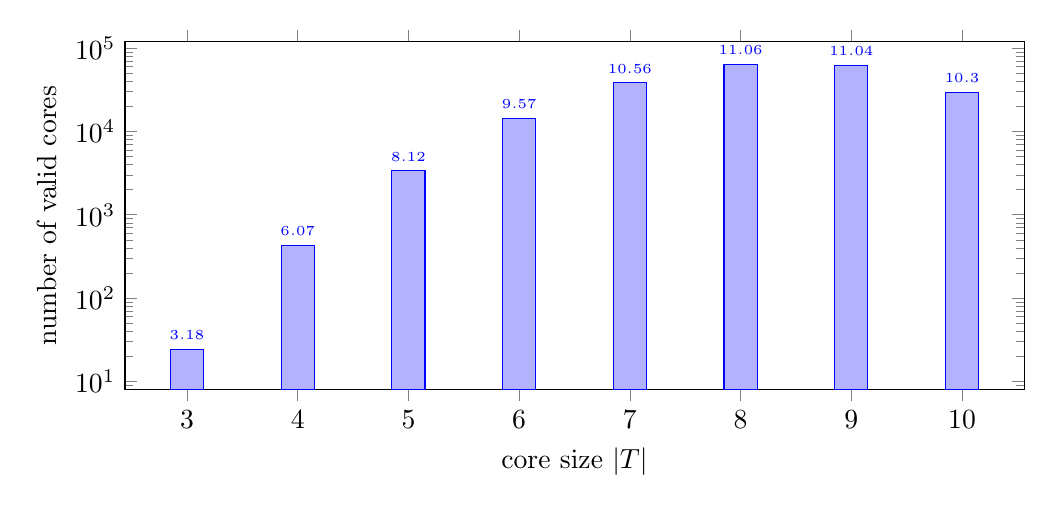
\begin{tikzpicture}
    \begin{axis}[
      ybar, bar width=12pt,
      width=13cm, height=6cm,
      ymode=log,
      log origin=infty,
      ymin=8, ymax=120000,
      symbolic x coords={3,4,5,6,7,8,9,10},
      xtick=data,
      xlabel={core size $|T|$},
      ylabel={number of valid cores},
      nodes near coords, nodes near coords style={font=\tiny},
      enlarge x limits=0.08,
    ]
    \addplot coordinates {(3,24) (4,432) (5,3360) (6,14400) (7,38400)
      (8,63488) (9,62464) (10,29696)};
    \end{axis}
  \end{tikzpicture}
  \caption{Hard-core size distribution of the $212{,}264$ valid $T$'s in
    Theorem~\ref{thm:factorization} [COMPUTED]$\times2$, log scale.  The
    $7{,}052{,}450$ minimal $u$-covers of~\eqref{eq:ucount} are the per-$T$
    singleton-fill products summed over these cores.}
  \label{fig:tcensus}
\end{figure}

\subsection{The forcing spectrum}
\label{sec:spectrum}

The sum identities are the spectrum's consistency core: $n_{\cH}=m$,
$n_{\cC}=C$, $n_{\cFh}+n_{\cFo}=F$, $n_{\cVh}+n_{\cVo}=35-\mathrm{cap}_2$,
$n_{\cH}+n_{\cC}=\mathrm{cap}_1$, $n_{\cC}+n_{\cFh}+n_{\cFo}=T$
(S1~\cite{D313}, definitional unfolding).

\begin{theorem}[S2(a)$'$ repaired forced-cell characterization; PROVED]
  \label{thm:s2ap}
  For $c\in U$:
  \begin{equation}
    \label{eq:s2ap}
    \sigma_S(c)\in\{\cFh,\cFo\}\iff
    c\in u(S)\land(\forall f\in S)(c\in\mathrm{covered}(f)\Rightarrow\neg p(f)):
    \texttt{s2a'\_forced}.
  \end{equation}
\end{theorem}

\begin{theorem}[S2(b--d); PROVED]
  \label{thm:s2bcd}
  For $c\in U$: $\sigma_S(c)\in\{\cH,\cC\}\iff(\exists f\in S)(p(f)\land
  c\in\mathrm{covered}(f))$ (pc-secured: \texttt{s2b\_pc});
  $\sigma_S(c)\in\{\cVh,\cVo\}\iff c\notin u(S)$ (\texttt{s2c\_void}); the
  hard/open split is exactly the $c\in\text{Hard6}$ check
  (\url{s2d_split}).
\end{theorem}

\begin{theorem}[S3 partition; PROVED]
  \label{thm:s3}
  The six classes~\eqref{eq:sig} partition $U$ (pairwise disjoint,
  exhaustive): \url{spectrum_partition}.  The ambiguous middle --- a
  cell covered both by a pc and by a composite-only family --- is resolved
  by the priority rule: pc-secured wins.
\end{theorem}

\begin{theorem}[S4 union monotonicity; PROVED]
  \label{thm:s4}
  With $\psi$ from~\eqref{eq:psi},
  \begin{equation}
    \label{eq:s4}
    \psi_{S\cup T}(c)=\max(\psi_S(c),\psi_T(c)):
    \texttt{psi\_union\_max}.
  \end{equation}
  Upgrades: $\cVh\to\cFh/\cH$, $\cVo\to\cFo/\cC$, $\cFh\to\cH$,
  $\cFo\to\cC$; $\{\cH,\cC\}$ absorbing.
\end{theorem}

Honest repair history.  S2(a) \emph{as originally stated} is false: its
right-hand side holds vacuously at every uncovered cell, misclassifying all
void cells as slack-forced (hostile review Q-53~\cite{D316}).  The repair
S2(a)$'$ restores the dropped conjunct $c\in u(S)$~\eqref{eq:s2ap}; the
failure set of the original is exactly the void cells --- $88{,}259$
(unweighted) pair-type$\times$cell checks fail, all at $c\notin u(S)$, zero
at covered cells [COMPUTED]$\times2$~\cite{D316}.  S2(b--d), S3, S4, and the
C1--C4 corollaries survived Q-53 unchanged~\cite{D316}.

The census (both paths, $3{,}081$ pair types, $\sum w=82{,}272{,}378$):
aggregate masses
\begin{equation}
  \label{eq:masses}
  \cH\,5.27\%,\ \cC\,26.66\%,\ \cFh\,6.41\%,\ \cFo\,35.15\%,\
  \cVh\,5.46\%,\ \cVo\,21.05\%,
\end{equation}
with $15.43\%$ of forced slack on hard cells ($\cFh/(\cFh+\cFo)$) --- hard
cells whose only coverage is composite-only, invisible to the aggregate $F$.
Upgrade anatomy over pair types: $18{,}948$ cell upgrades
($\cVh\!\to\!\cH$ $1616$, $\cVh\!\to\!\cFh$ $1616$, $\cVo\!\to\!\cC$ $7682$,
$\cVo\!\to\!\cFo$ $7540$, $\cFh\!\to\!\cH$ $89$, $\cFo\!\to\!\cC$ $405$):
$F\!\to\!$pc ``rescues'' are rare ($494$)~\cite{D313,D316}.  Cell-level:
cell~$0$ has the lowest $\cH$ mass of the six hard cells ($30.31\%$ vs
$30.75\%$ hard mean, quantifying the no-surgical-group gap); cell~$16$ is
covered in $92.3\%$ of pairs but pc-secured in only $30.27\%$~\cite{D313,D316}.
All [COMPUTED]$\times2$.  (Terminology note: ``forcing spectrum'' denotes
something unrelated in matching-forcing theory~\cite{AMM04}; the qualified
name \emph{ES} forcing spectrum avoids the collision~\cite{D313}.)

\begin{figure}[t]
  \centering
  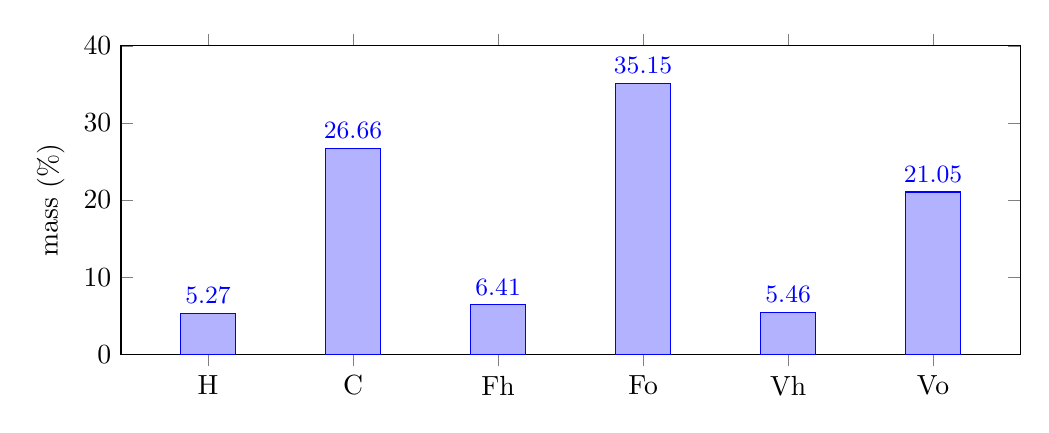
\begin{tikzpicture}
    \begin{axis}[
      ybar, bar width=20pt,
      width=13cm, height=5.5cm,
      ymin=0, ymax=40,
      symbolic x coords={H,C,Fh,Fo,Vh,Vo},
      xtick=data,
      ylabel={mass (\%)},
      nodes near coords, nodes near coords style={font=\small},
      enlarge x limits=0.12,
    ]
    \addplot coordinates {(H,5.27) (C,26.66) (Fh,6.41)
      (Fo,35.15) (Vh,5.46) (Vo,21.05)};
    \end{axis}
  \end{tikzpicture}
  \caption{Aggregate six-class masses~\eqref{eq:masses} of the ES forcing
    spectrum over the pair census ($3{,}081$ pair types,
    $\sum w=82{,}272{,}378$) [COMPUTED]$\times2$.  The spectrum strictly
    refines $(T,F,C)$: $35$ of $48$ distinct $(T,F,C)$ triples admit $\ge2$
    distinct spectra~\cite{D313}.}
  \label{fig:spectrum}
\end{figure}

\subsection{The forcing decomposition A--D}
\label{sec:adecomp}

The two-sided forcing decomposition of the R281 census~\cite{D322} is
formalized as [PROVED]:
\begin{itemize}
\item \textbf{Theorem A} (open--hard coincidence): $n=24k+1\equiv H\pmod{840}
  \iff k\equiv(H-1)/24\pmod{35}$ for the six hard classes
  (\texttt{theoremA\_crt}, \texttt{decide}); the six $k$-classes are exactly
  $k\bmod7\in\{0,1,5\}\times k\bmod5\in\{0,2\}$
  (\url{theoremA_crt_box}).
\item \textbf{Theorem B} (scaling-forced composites): a solution of
 ~\eqref{eq:es} for $n$ scales to one for $kn$ (\texttt{theoremB\_scaling},
  field algebra).
\item \textbf{Theorem C} (filter = $F$-axis): definitional unfolding
  (\url{theoremC_filter}).
\item \textbf{Theorem D} (surgical characterization): divisor analysis plus
  \texttt{decide} (\url{theoremD_card}, \url{theoremD_mod7},
  \url{theoremD_surgical}).
\end{itemize}
The Q-25 review verdict (SURVIVES conditional~\cite{D322}) binds the
following conditions, stated verbatim from the module docstrings:
(1) B's Reading carries the prime-free-class lemma: every non-prime-covering
class is prime-free, i.e.\ $\gcd(24k_0+1,24\cdot\mathrm{mprime})>1$ ---
certified $8{,}965/8{,}965$ on the census data, NOT proved in general.  B
alone does not make $F$ forced.
(2) `prime-covering' $:=$ R7's $x\cdot h$ criterion.  The `$C=$ prime
coverage' glosses are dropped: $262$ pc families are prime-free, and $38.2\%$
of $C$ units lie in cell sub-progressions with no primes.
(3) Aggregate slack is stated as unweighted cell hits ($m$ counts cells hit,
not density; the density-weighted $F$ share is $55.0\%$, not $68.3\%$).
(4) R7 tests $ab\mid x\cdot h$, NOT $\mathrm{lcm}(a,b)\mid x\cdot h$
($5{,}582$ families pass the lcm test; the $1{,}720$ extra are all
prime-free).

%======================================================================
\section{Discussion}
%======================================================================

\paragraph{The census poset's shape.}  The $78$ groups are
[COMPUTED]$\times2$ data~\cite{D304}: $303$ strict absorption pairs; unique
maximal element $\top=(\mathbb{Z}/35,1)$ with $1{,}945$ families (every group
$\preceq\top$); $29$ minimal elements ($25$ composite-only singletons plus
$4$ prime-covering singletons on non-hard cells); height $4$, width $39$
(Table~\ref{tab:census}, Figure~\ref{fig:hasse}).  Deeper structure~\cite{D308}:
rank distribution $29/35/13/1$ (ranks $0$--$3$), $164$ covers with $8$
``jump'' covers (rank-$0\lessdot$rank-$2$), hence the poset is \emph{not}
graded.  The census poset is a join-semilattice ($6{,}084/6{,}084$ joins;
abstract join in census only $870/6{,}084$) but not a lattice ($1{,}054/6{,}084$
meets)~\cite{D308}.  Minimal Hard6 prime-covers number exactly $16$, all
antichains (A3 audit); surgical-only coverage is impossible since cell~$0$
carries no singleton~\cite{D308}.  The $8.9\times10^{13}$ antichains
(single-path count) collapse to $212{,}264$ hard cores under the singleton
factorization of Theorem~\ref{thm:factorization} --- the count~\eqref{eq:ucount}
closes the open Z35 minimal-$u$-cover enumeration~\cite{D308,D312}.

\begin{figure}[t]
  \centering
  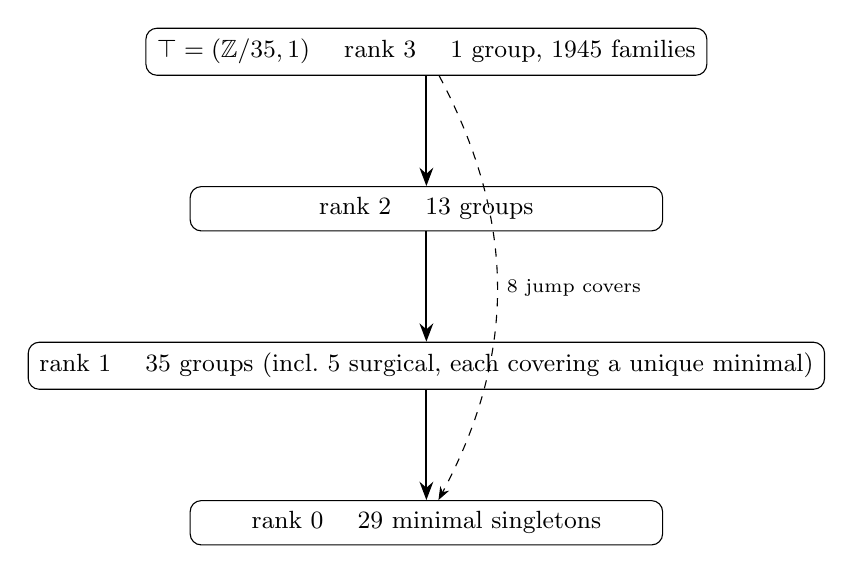
\begin{tikzpicture}[node distance=1.4cm,
      every node/.style={font=\small},
      box/.style={draw, rounded corners, minimum width=6cm, align=center,
        inner sep=4pt}]
    \node[box] (top) {$\top=(\mathbb{Z}/35,1)$ \quad rank $3$ \quad
      $1$ group, $1945$ families};
    \node[box, below=of top] (r2) {rank $2$ \quad $13$ groups};
    \node[box, below=of r2] (r1) {rank $1$ \quad $35$ groups
      (incl.\ $5$ surgical, each covering a unique minimal)};
    \node[box, below=of r1] (r0) {rank $0$ \quad $29$ minimal singletons};
    \draw[-{Stealth}, thick] (top) -- (r2);
    \draw[-{Stealth}, thick] (r2) -- (r1);
    \draw[-{Stealth}, thick] (r1) -- (r0);
    \draw[-{Stealth}, dashed, bend left=28] (top) to
      node[right, font=\scriptsize]{$8$ jump covers} (r0);
  \end{tikzpicture}
  \caption{Schematic of the census absorption poset (not to scale):
    counts are exact [COMPUTED]$\times2$~\cite{D304,D308}.  Every group
    absorbs into the unique top $\top$; surgical rank-$1$ groups sit atop
    their unique minimal cell-mates (A4's down-set is the
    [OPEN] item of~\S\ref{sec:absorp}).}
  \label{fig:hasse}
\end{figure}

\begin{table}[t]
  \centering
  \caption{Selected census facts [COMPUTED]$\times2$~\cite{D304,D308,D312,D313,D316}.}
  \label{tab:census}
  \begin{tabular}{ll}
    \toprule
    quantity & value \\
    \midrule
    union groups & $78$ \\
    strict absorption pairs & $303$ \\
    top group $(\mathbb{Z}/35,1)$ families & $1{,}945$ \\
    minimal elements & $29$ \\
    height / width & $4$ / $39$ \\
    covers (rank-$0\lessdot$rank-$2$ jumps) & $164$ ($8$) \\
    census joins / meets & $6{,}084$ / $1{,}054$ \\
    surgical groups (cells $5,7,12,15,22$) & $5$, down-set size $2$ each \\
    valid hard cores $T$ & $212{,}264$ \\
    minimal $u$-covers of $\mathbb{Z}/35$ & $7{,}052{,}450$ \\
    singleton groups / singleton-cells & $52$ / $29$ \\
    spectrum pair types / weighted pairs & $3{,}081$ / $82{,}272{,}378$ \\
    \bottomrule
  \end{tabular}
\end{table}

\paragraph{The greedoid episode, honestly labeled.}  Beyond the formalized
core, the program developed a greedoid-level theory on the poset~\cite{D311}:
both candidate feasible families satisfy accessibility (D1); exchange fails
for both, witnessed by $X=\{4,5\}$, $Y=\{\top\}$ (D2); the failure is exactly
characterized by the comparability shadow (D3), also failing with no top in
sight ($X=\{4,6\}$, $Y=\{0\}$, D3$'$); and the redundancy rank refutes core
canonicity: $S=\{0,4,6,17,22,29,35,38\}$ has exactly two cores, $\{0\}$ and
the seven singletons, so $\rho(S)=7$ (R5).  These all SURVIVED hostile review
Q-48~\cite{D315} but are \emph{not Lean-formalized}: we report them as
[PROVED*] context, not as claimed theorems of this paper.

\paragraph{Lessons from the two objections.}  The Q-48 objection~\cite{D315}
showed the naive R3 proof transferred a reduction sequence across the
$S\cap T\ne\emptyset$ boundary where it cannot transfer; the disjoint
restriction is not a weakening of convenience but the true statement, and
the general corollary R3$''$ plus the deficit bound~\eqref{eq:deficitbound}
say exactly how much overlap can destroy.  The Q-53 objection~\cite{D316}
showed a dropped conjunct ($c\in u(S)$) silently universalized a
characterization to cells where its hypothesis was vacuous.  Both repairs
survived re-review (Q-55, Q-56~\cite{D322}).

\paragraph{Limitations.}  (i) The Lean theorems quantify over abstract
$(C,p)$ data; transfer to the $78$-group census rests on the reconstruction
fidelity of Assumption~\ref{asm:census}, not on a machine-checked census.
(ii) The spectrum census~\eqref{eq:masses} describes the R281 census
universe, not general ES theorems~\cite{D316}.  (iii) The deficit bound is
one-sided; no exact $\delta(S,T)$ formula is known, and maximal
exchange-closed subfamilies are open~\cite{D315,D311}.  (iv) The monotone
R59/R63 audit of all proofs is a human audit, not a machine check.
(v) A4 is [OPEN]; minimal-cover enumeration beyond the group level (Q-30's
family-level machinery) is a disjoint layer, not pursued here~\cite{D312}.

%======================================================================
\section{Conclusion}
%======================================================================

We have given the union layer of the Erd\H{o}s--Straus covering program an
order theory and a cellwise forcing profile, both machine-checked.  The
absorption order $\preceq$ of~\eqref{eq:absorp} is a partial order
(Theorem~\ref{thm:a1}) that characterizes datum-equality
(Theorem~\ref{thm:a2}) and prunes dominated families while preserving the
datum (Theorem~\ref{thm:a3}).  The redundancy rank $\rho$ of~\eqref{eq:rho}
satisfies disjoint superadditivity (Theorem~\ref{thm:r3p}), its general
corollary (Theorem~\ref{thm:r3pp}), the one-sided overlap-deficit bound
(Theorem~\ref{thm:tb}), and the absorption-collapse formula with uniqueness
(Theorem~\ref{thm:r4p}) --- with the naive unrestricted superadditivity
honestly refuted (Proposition~\ref{prop:r3refuted}).  The singleton
factorization (Theorem~\ref{thm:factorization}) reduces the minimal
$u$-cover census of $\mathbb{Z}/35$ to a $2^{24}$ factorization yielding the
exact count $7{,}052{,}450$.  The ES forcing spectrum~\eqref{eq:sig} carries
the repaired forced-cell characterization (Theorem~\ref{thm:s2ap}), the
pc-secured/void/split laws (Theorem~\ref{thm:s2bcd}), the six-class
partition (Theorem~\ref{thm:s3}), and the union-max rule (Theorem~\ref{thm:s4}),
together with its complete pair-type census.  Theorems~A--D close the cited
two-sided decomposition under four documented conditions.  All of this is
[COMPUTED]$\times2$ where data and [PROVED] where mathematics, except the
surgical down-set A4, which we leave explicitly [OPEN].

%======================================================================
\section{References}
%======================================================================

\begin{thebibliography}{9}

\bibitem{Erd50}
P.~Erd\H{o}s,
\emph{On a Diophantine equation},
Mat.\ Lapok \textbf{1} (1950), 192--210.
(The Erd\H{o}s--Straus conjecture.)

\bibitem{Mor69}
L.~J.~Mordell,
\emph{Diophantine Equations},
Academic Press, 1969.
(Theorem~A's CRT computation; Mordell's list of admissible squares
mod~$840$.)

\bibitem{AMM04}
P.~Adams, M.~Mahdian, and E.~S.~Mahmoodian,
\emph{On the forced matching numbers of bipartite graphs},
Discrete Math.\ \textbf{281} (2004), 1--12.
(``Forcing spectrum'' in matching-forcing theory is an unrelated object;
our qualified name \emph{ES} forcing spectrum avoids the collision.)

\bibitem{D304}
D.~Blair,
\emph{Unsolved Math --- Round 304: the ES absorption poset},
program dossier, 2026-10-11.
(Supplied datum: $78$-group census; A1--A4, Q-46 SURVIVES.)

\bibitem{D308}
D.~Blair,
\emph{Unsolved Math --- Round 308: absorption-poset antichains, redundancy
\& lattice structure},
program dossier, 2026-10-11.
(Supplied datum: B1/B2, join-semilattice, minimal Hard6 covers.)

\bibitem{D311}
D.~Blair,
\emph{Unsolved Math --- Round 311: the cover greedoid of the ES absorption
poset},
program dossier, 2026-10-11.
([PROVED*] D1--D3, R1--R5; Q-48 SURVIVES for all but R3/R4's wording.)

\bibitem{D312}
D.~Blair,
\emph{Unsolved Math --- Round 312: Z35 minimal $u$-cover census via
singleton-factorization},
program dossier, 2026-10-11.
(Supplied datum: $212{,}264$ cores, $7{,}052{,}450$ covers
[COMPUTED]$\times2$; Q-52 SURVIVES.)

\bibitem{D313}
D.~Blair,
\emph{Unsolved Math --- Round 313: ES forcing spectrum},
program dossier, 2026-10-11.
(Supplied datum: spectrum census $3{,}081$ pair types; S1--S4/C1--C4,
Q-53 SURVIVES except S2(a) as stated.)

\bibitem{D314}
D.~Blair,
\emph{Unsolved Math --- Round 314: Lean + rule-9 lane},
program dossier, 2026-10-11.
(Supplied datum: Q-46 quoted SURVIVES verdict.)

\bibitem{D315}
D.~Blair,
\emph{Unsolved Math --- Round 315: repair of the cover-greedoid theory
after Q-48},
program dossier, 2026-10-11.
(Supplied datum: R3 refutation, R3$'$/R3$''$/T/R4$'$ repairs, Q-48 quoted
OBJECTION verbatim.)

\bibitem{D316}
D.~Blair,
\emph{Unsolved Math --- Round 316: ES forcing-spectrum S2(a) repair (after
Q-53 OBJECTION)},
program dossier, 2026-10-11.
(Supplied datum: S2(a)$'$ repair, $88{,}259$-check failure census,
Q-53 quoted OBJECTION verbatim.)

\bibitem{D322}
D.~Blair,
\emph{Unsolved Math --- Round 322: Lean + rule-9 lane (fold complete)},
program dossier, 2026-10-11.
(Supplied datum: $34$-theorem bakkie build --- exit $0$, zero sorrys,
standard axioms; Q-25 SURVIVES conditional with four conditions; Q-55 and
Q-56 quoted SURVIVES verdicts.)

\end{thebibliography}

\end{document}

%======================================================================
% SELF-REVIEW (author's notes, not part of the paper)
%======================================================================
% SUBSTANTIVE WEAKNESSES
% 1. Transfer gap (Assumption~\ref{asm:census}): the Lean theorems are proved
%    over abstract (C,p) data, while every census number in the paper rests
%    on the fidelity of the 78-group / 3,081-pair-type reconstructions. No
%    machine-checked bridge exists between the two layers; if a reconstruction
%    is wrong, the paper's census-backed claims (e.g. Theorem~\ref{thm:tb}'s
%    sharpness witness, the strictness witnesses of~\S\ref{sec:rho}) lose
%    their examples while the theorems themselves still hold abstractly.
% 2. The overlap-deficit bound (Theorem~\ref{thm:tb}) is one-sided: no exact
%    formula for \delta(S,T) in terms of overlap structure is known, so the
%    "answer" to when superadditivity breaks is necessary/sufficient
%    conditions plus a bound, not a characterization. The deficit can even be
%    negative, so the bound says little in the interesting direction.
% 3. The R59/R63 monotone audit is a human audit recorded in the dossiers,
%    not a machine check; and the D1--D3''/R1/R5 material reported in
%    Discussion is [PROVED*] but not Lean-formalized, so the paper's honest
%    center of gravity (the formalized core) is thinner than the full theory
%    the dossiers built. A4 remains [OPEN], leaving the surgical layer of the
%    poset theory incomplete.
% TYPOGRAPHY ISSUES
% 1. Table~\ref{tab:lean} puts long Lean theorem names in a fixed-width
%    p-column; {\small\url{...}} was needed throughout to keep lines from
%    overrunning the column (verify with overfull-\hbox logs at build time).
% 2. The six spectrum-class macros (\cH, \cC, \cFh, \cFo, \cVh, \cVo) are set
%    upright in \textnormal so they do not collide with italic math symbols
%    or with the calligraphic C used for covered cells; in the pgfplots bar
%    chart these macros expand inside symbolic x coords and must remain
%    brace-safe (they are, but redefinition elsewhere would break it).
% 3. \ref forward references (Theorem~\ref{thm:s4} is cited from the
%    Abstract) and the ucount/masses equation cross-references
%    need at least two LaTeX passes; latexmk handles this, but a single
%    pdflatex run will leave ?? markers in the Abstract.
%======================================================================
